\subsection{Абстрактный синтаксис}
Описание языка в среде "<MPS"> обычно начинается с задания абстрактного синтаксиса \cite{redDragon} этого языка. Для этого в среде "<MPS"> предусмотрен специальный проблемно-ориентированный язык "<jetbrains.mps.bootstrap.structureLangauge"> (далее "<structureLanguage">). Этот язык позволяет описать концепты языка и отношения между ними. С помощью этого же языка задаются свойства и мета-свойства концептов. Весь абстрактный синтаксис языка описывается в модели "<structure"> этого языка.

Для объявления пользовательских концептов в языке "<structureLangauge"> определен концепт "<ConceptDeclaration">. Например, корневой узел, описывающий концепт "<StateMachine">, предствлен на рисунке \ref{fig:StateMachineConcept}.

\begin{figure}
\centering
\fbox{
 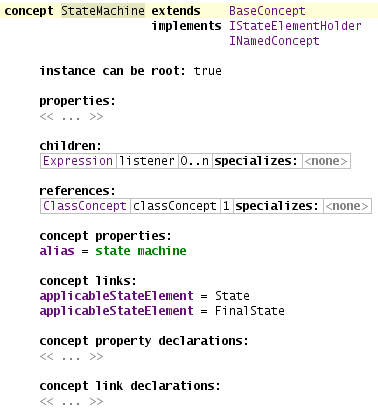
\includegraphics[width=0.9\textwidth]{StateMachineConcept.png}
}
\caption{Объявление концепта "<StateMachine">}
\label{fig:StateMachineConcept}
\end{figure}


Из рисунка видно, что объявление концепта состоит из нескольких секций:
\begin{itemize}
 \item секция "<concept StateMachine"> задает имя концепта;

 \item секция "<extends BaseConcept"> указывает на то, что концепт является расширением концепта "<BaseConcept">.
 Отношение расширения в языке "<structureLanguage"> имеет тот же смысл, что и в традиционных объектно-ориентированных
 языках программирования: если концепт "<B"> является расширением концепта "<A">, то все экземпляры концепта "<B">
 являются также и экземплярами концепта "<A">. Так же концепт "<B"> наследует все свойства и отношения концепта
 "<A">.  Каждый концепт объявленный в среде "<MPS"> является прямым или косвенным расширением концепта
 "<BaseConcept">,  также как в языке "<Java"> все классы прямо или косвенно расширяют класс "<java.lang.Object">;

 \item в секции "<implements IStateElementHolder INamedConcept"> перечислены интерфейсы-концепты реализуемые
 концептом "<StateMachine">. Понятие "<интерфейса-концепта"> ближе всего к понятию "<trait"> языка "<Scala"> [ссылка].
 Интерфейс-концепт также может иметь свойства и отношения с другими концептами. При этом не может быть узлов,
 являющихся непосредственными экземплярами интерфейса-концепта. Интерфейсы-концепты полезны для создания неполного
 множественного наследования: концепт наследует все свойства и отношения тех интерфейсов-концептов, которые он
 реализует;

 \item в секции "<instance can be root"> задается могут ли экземпляры концепта быть корневыми узлами моделях. В
 данном случае, экземпляры концепта "<StateMachine"> могут быть корневыми;

 \item в секции "<properties"> перечисляются свойства, которые может иметь экземпляр концепта. Концепт "<StateMachine"> не определяет собственных свойств, однако у экземпляров этого концепта может быть задано свойство "<name">, унаследованное от интерфейса-концепта "<INamedConcept">;

 \item в секции "<children"> описывается структура вложенных узлов. Для каждого элемента в этой секции задается концепт, роль и арность вкладываемых узлов. Арность определяет ограничение на количество вложенных экземпляров данного концепта с данной ролью. Арность может быть задана одним из четырех значений:
\begin{description}
 \item["<1">] ровно один экземпляр;
 \item["<0..1">] не более одного экземпляра;
 \item["<1..n">] хотя бы один экземпляр;
 \item["<0..n">] произвольное количество экземпляров.
\end{description}
Например, в экземпляр концепта "<StateMachine"> может быть вложено произвольное количество экземпляров концепта "<Expression"> с ролью "<listener">. Кроме этого экземпляр концепта "<StateMachine"> может содержать произвольное количество вложенных экземпляров интерфеса-концепта "<IStateElement">, так как в секции "<children"> интерфейса-концепта "<IStateElementHolder"> есть элемент "<IStateElement stateElement 0..n">, и концепт "<StateMachine"> реализует интерфейс-концепт "<IStateElementHolder">;

\item в секции "<references"> определяется структура ссылок концепта. Также, как и в случае вложенных узлов, каждый элемент в этой секции задает целевой концепт, роль и арность ссылки. Арность ссылки может быть задана одним из двух значений:
\begin{description}
 \item["<1">] обязательная ссылка;
 \item["<0..1">] необязательная ссылка.
\end{description}
Например, каждый экземпляр концепта "<StateMachine"> должен иметь ссылку с ролью "<classConcept"> на экземпляр концепта "<ClassConcept">;

\item четыре последних секции предназначены для описания мета-структы концепта. в секции "<concept properties"> задаются значения мета-свойства концепта. Для концепта "<StateMachine"> значение мета-свойства "<alias"> определено как "<state machine">. Это специальное мета-свойство, значение которого используется средой "<MPS"> в качестве имени концепта в пользовательском интерфейсе. Например, в меню создания корневого узла, опция, соответствующая созданию экземпляра концепта "<StateMachine">, будет называться "<state machine"> (Рис. \ref{fig:CreateStateMachine}).

\begin{figure}
 \centering
 \fbox{
  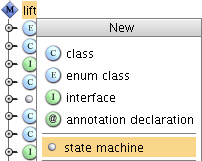
\includegraphics{CreateStateMachine.png}
 }
 \caption{Меню создания корневого узла}
 \label{fig:CreateStateMachine}
\end{figure}

В секции "<concept links"> задаются значения мета-отношений концепта. В секциях "<concept property declaration"> и "<concept link declarations"> объявляются мета-свойства, значения которых могут быть заданы в самом концепте или в расширяющих его концептах. Например, в интерфейсе-концепте "<IStateElementHolder"> объявлено мета-отношение "<applic\-able\-Sta\-te\-Ele\-ment">, значение которого используется в языке "<stateMachine"> для того, чтобы уточнить какие именно автоматные конструкции могут быть вложены в другие автоматные конструкции. Значения
$$
\begin{array}{l}
applicableStateElement = State\\
applicableStateElement = FinalState
\end{array}
$$
для концепта "<StateMachine"> указывают на то, что автомат может содержать обычные и конечные состояния.
\end{itemize}

Абстрактный синтаксис языка может быть представлен виде UML-диаграммы классов \cite{uml}. Для языка "<stateMachine"> такая диаграмма приведена на рисунке \ref{fig:AbstractSyntax}.

\begin{figure}
 \centering
 \fbox{
  
\includegraphics{AbstractSyntax.png}
 }
 \caption{Абстрактный синтаксис языка "<stateMachine">}
 \label{fig:AbstractSyntax}
\end{figure}
